\section{Experimental Evaluation}
\label{sec:exp}

To demonstrate the practical value of our approach to refinement checking,
we argue that our $k$-approximation:
\begin{itemize}

  \item uncovers violations with small values of $k$,

  \item can be efficiently implemented for use in systematic concurrency
  testing and long-term runtime monitoring, and
  
  \item can be efficiently implemented for use in static analysis.

\end{itemize}

To argue these points, we have studied actual concurrent data structure
implementations in C/C++, including the
Scal\footnote{\url{http://scal.cs.uni-salzburg.at}} High-Performance
Multicore-Scalable Computing suite. Some of these implementations, such as the
Michael-Scott Queue~\cite{conf/podc/MichaelS96}, are meant to preserve
observational refinement\footnote{More precisely, they have been designed to be
linearizable.}, while others, such as Kirsch et al.'s
$k$-FIFO~\cite{conf/pact/KirschLP13}, are meant to preserve weaker properties.
Unless otherwise noted, we use these implementations without modification,
except to annotate methods with a fixed set of possible preemption points,
e.g.,~preceding shared-memory accesses.

For our first two experiments (\S\ref{sec:exp:coverage},
\S\ref{sec:exp:dynamic}), we have developed a tool for enumerating a (possibly
large) number of alternate executions involving a limited number of object
method invocations. We run each operation on a separate thread, and execute all
thread schedules up to a given number $n \in \<Nats>$ of thread preemptions, at
specified preemption points, similarly to Microsoft's Chess
tool~\cite{conf/osdi/MusuvathiQBBNN08}. With $n=0$ preemptions, there is only
one schedule to execute, though the number of schedules grows exponentially as
$n$ increases. For instance, with our annotation of preemptions in Scal's
Michael-Scott Queue, we execute $f(n)$ schedules of a program with $8$ method
invocations at a rate of roughly one million schedules per minute, where $f$ is
given by
{\footnotesize
\begin{align*}
  f(1) = 33, f(2) = 612, f(3) = 8343, f(4) = 95434, f(5) = 930141
\end{align*}}%
While similar in spirit to the second, our third experiment
(\S\ref{sec:exp:static}) executes all round-robin thread schedules up to a
given number $n \in \<Nats>$ of rounds \emph{symbolically}: we use
CSeq~\cite{conf/ase/FischerIP13} to sequentialize a simple program which
invokes a limited number of library methods, and then
CBMC~\cite{conf/tacas/KroeningT14} (version 4.5) to perform bounded model
checking up to a given loop-unroll bound. All measurements were made on similar
MacBook Pro 2.XGHz Intel Core i5/i7 machines. While space prohibits including
the entirety of our experiments, we do include a representative sample and
analysis.

\subsection{Coverage of Refinement Violations}
\label{sec:exp:coverage}

To show that our approximation $A_k$ uncovers observational refinement
violations with small values of $k$, we measure the number of history
violations detected by a traditional linearizability checker\footnote{We
implement a linearization-enumerating monitor, as in
Line-Up~\cite{conf/pldi/BurckhardtDMT10}.\label{fn:lineup}} versus those caught
by $A_k$. The linearizability checker serves as an exact measure due to the
equivalence of Section~\ref{sec:lin}. While the approximation $A_k(H(e))$ of a
violation $H(e)$ may not itself be a violation, one hopes to encounter some
execution $e'$ for which the violation $A_k(H(e'))$ \emph{covers} $H(e)$,
i.e.,~for which $A_k(H(e')) \preceq H(e)$.

Figure~\ref{fig:data:coverage} demonstrates that $A_k$ covers most or all
violations with small values of $k$. While $A_4$ suffices to cover all
violations at nearly all data points --- besides the first point, where the
sample size of $1023$ executions is small relative to the $8$ operations ---
all values $k > 0$ capture a nontrivial and increasing number of violations. In
fact, as the execution-sample size increases (the x-axis is ordered by number
of executions over operations) the value of $k$ required to capture a violation
appears to decrease, all violations being captured by $A_3$ after a certain
point. Note that this data set only exhibits \emph{order violations} (see
Section~\ref{sec:containers}), i.e.,~where elements are removed out of order;
in general, there is no cutoff value of $k \in \<Nats>$ for which all
\emph{empty violations} can be captured with $A_k$.

\begin{figure}
  \centering
  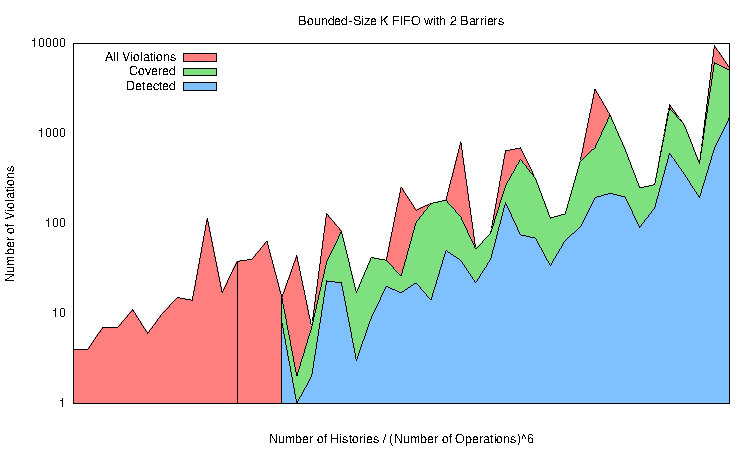
\includegraphics[width=\linewidth]{figures/coverage-bkq-2-barriers}
  \caption{Comparison of violations covered with
    $k \le 4$. Each data point counts histories on a logarithmic scale over
    all executions up to $5$ preemptions on Scal's nonblocking
    bounded-reordering queue with $i \le 4$ enqueue operations and $j \le 4$
    dequeue operations. The x-axis is ordered by increasing number of
    executions ($1023$--$2359292$) over $i\!+\!j$; we show only points with over
    $1000$ executions. The largest data points measure the total
    number of unique histories encountered over a given set of executions.
    Second are the number of those histories violating refinement.
    Following are the
    numbers of those violations covered by $A_k$, for varying values of $k$.
  }
  \label{fig:data:coverage}
\end{figure}

\subsection{Operation Counting for Testing \& Runtime Monitoring}
\label{sec:exp:dynamic}

Figure~\ref{fig:data:runtime} compares the runtime overhead of our $A_2$
approximation versus a traditional linearizability checker\footnote{See
footnote~\ref{fn:lineup}.} sampling executions with up to $20$ operations on
Scal's nonblocking Michael-Scott queue. Since computing the set $\ker
H(L_\mathrm{msq})$ of sequential histories over $n$ operations becomes
prohibitively expensive as $n$ increases, surpassing a timeout of $5$m for
$n\!=\!7$, we bypass the computation of $\ker H(L_\mathrm{msq})$ entirely,
simply enumerating the linearizations of a given execution history without
checking its inclusion. Despite our best-effort implementation, one observes
the cost incurred by linearization: as the number of operations increases, the
number of linearizations increases exponentially, and performance plummets.
With only 20 operations, instrumentation overhead is nearly 100000\%. Our
counting-based implementation of $A_2$ avoids this dramatic overhead: though
not seriously optimized, we observe that runtime overhead stays within 30\%.
This scalability suggests that our approximation can be used not only for
systematic concurrency testing with few method invocations, but also for
runtime monitoring, where the number of operations grows without limit.

\begin{figure}
  \centering
  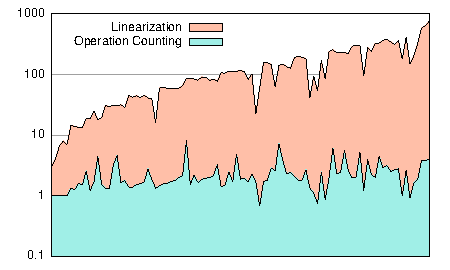
\includegraphics[width=\linewidth]{figures/lin-vs-counting-time}
  \caption{Comparison of runtime overhead between linearization-based monitoring
    and operation counting (for $A_2$) for up to $20$ operations. Each data
    point measures runtime on a \textbf{logarithmic scale}, normalized to
    unmonitored execution time, over all executions up to $3$ preemptions on
    Scal's nonblocking Michael-Scott queue with $i\!\le\!10$ enqueue operations
    and $j\!\le\!10$ dequeue operations. The x-axis is ordered by increasing
    $i\!+\!j$, and each data point is sampled from up to $126600$ executions.
    Times do not include pre-calculation of sequential histories for
    linearization-based monitoring. While our $A_k$ monitor
    scales well, maintaing under 30\% overhead, the linearization monitor
    scales \textbf{exponentially}, running with roughly \textbf{100000\%
    overhead} with $20$ operations.
  }
  \label{fig:data:runtime}
\end{figure}

\subsection{Operation Counting for Static Analysis}
\label{sec:exp:static}

Our approximation $A_k$ also leads to an effective static means of detecting
refinement violations, due to the simplicity of an operation-counting based
implementation. Essentially, by using only simple increment and decrement
operations on integer counters, we are able to leverage static verification
tools that are capable of integer reasoning. We have found that the major
obstacle in leveraging such tools is concurrency: even though the required
counter reasoning is simple, reasoning precisely about program concurrency is a
formidable challenge, with or without our operation-counting instrumentation.

Despite the difficultly of concurrency reasoning statically, we have
successfully applied our approach using two different static-verification
backends: one based on SMACK~\cite{conf/cav/RakamaricE14} and
Corral~\cite{conf/cav/LalQL12}, and the other based on
CSeq~\cite{conf/ase/FischerIP13} and CBMC~\cite{conf/tacas/KroeningT14}. Both
toolchains are based on sequentialization~\cite{journals/fmsd/LalR09} and
SMT-based bounded model checking. Our results in Table~\ref{tab:exp:static}
report only on the latter toolchain. Among $5$ data structure implementations,
we manually injected $9$ realistic concurrency bugs. All bugs were uncovered as
refinement violations with approximation $A_0$ or $A_1$, in round-robin
executions of up to $4$ rounds, of a program with at most $4$ {\sf push} and
$4$ {\sf pop} operations, and with loops unrolled up to $2$ times. Although the
time complexity of concurrent exploration is high independently of our
operation-counting instrumentation, particularly as the number of rounds
increases, one clearly observes that our approximation is effective in
detecting violations statically.

\begin{table}[t]
  \footnotesize
  \centering
  \begin{tabular}{llllllr}
  Library & Bug                  & $P$ & $k$ & $m$ & $n$ & Time \\
  \hline
  %MSQueue                             & 2xEnqueue 2xDequeue & 0 & 2 & 2 & & Yes \\
  Michael-Scott Queue & $\text{B}_1$ ({\tt head}) & $2\x2$ & 1 & 2 & 2 & 24.76s \\
  Michael-Scott Queue & $\text{B}_1$ ({\tt tail}) & $3\x1$ & 1 & 2 & 3 & 45.44s \\
  Treiber Stack & $\text{B}_2$              & $3\x4$ & 1 & 1 & 2 & 52.59s \\
  Treiber Stack & $\text{B}_3$ ({\tt push})       & $2\x2$ & 1 & 1 & 2 & 24.46s \\
  Treiber Stack & $\text{B}_3$ ({\tt pop})        & $2\x2$ & 1 & 1 & 2 & 15.16s \\
  Elimination Stack & $\text{B}_4$          & $4\x1$ & 0 & 1 & 4 & 317.79s \\
  Elimination Stack & $\text{B}_5$             & $3\x1$ & 1 & 1 & 4 & 222.04s \\
  Elimination Stack & $\text{B}_2$          & $3\x4$ & 0 & 1 & 2 & 434.84s \\
  Lock-coupling Set & $\text{B}_6$        & $1\x2$ & 0 & 2 & 2 & 11.27s \\
  LFDS Queue & $\text{B}_7$           & $2\x2$ & 1 & 1 & 2 & 77.00s   
  \end{tabular} 
  \caption{Runtimes for the static detection of injected refinement violations
    with CSeq \& CBMC. For a given program $P_{i\x j}$ with $i$ and $j$
    invocations to the {\sf push} and {\sf pop} methods, we explore the
    $n$-round round-robin schedules of $P_{i\x j}$ with $m$ loop iterations
    unrolled, with a monitor for our $A_k$ approximation. Bugs are
    ($\text{B}_1$)~non-atomic lock operation, ($\text{B}_2$)~ABA
    bug~\cite{tr/ibm/Michael04}, ($\text{B}_3$)~non-atomic CAS operation,
    ($\text{B}_4$)~misplaced brace, ($\text{B}_5$)~forgotten assignment,
    ($\text{B}_6$)~misplaced lock, ($\text{B}_7$)~predetermined capacity
    exceeded.
  }
  \label{tab:exp:static}
\end{table}

%% NOTE THE FOLLOWING IS GOOD TO KNOW EVEN IF IT DOESN'T APPEAR IN THE PAPER
%
% MSQueue (Michael \& Scott two-lock concurrent
% queue~\cite{conf/podc/MichaelS96}) uses a different lock for the head and
% respectively the tail of the singly-linked list used to store queue elements
% (Enqueuers access only the tail while Dequeuers access only the head). We have
% replaced the lock on the head (resp., tail) with a faulty lock, which enables
% two concurrent Dequeues (resp, Enqueue's) to try and update the queue at the
% same time, resulting in a lost update.
%
% For the Treiber Stack, we created a version where the memory management is
% done manually (using an array), in order to expose the well-known ABA bug{} to
% the CBMC backend. With this change, CSeq was able to detect the ABA bug{},
% using 3 {\sf push}'s, and 4 {\sf pop}'s. After fixing the ABA bug{} by
% removing a {\sf free} operation, we inserted two atomicity bugs, one in the
% {\sf push} method, one in the {\sf pop} method, resulting as for the MSQueue
% in lost updates (and thus linearizability violations).
%
% The Elimination Stack \citep{conf/spaa/HendlerSY04} uses the Treiber Stack as
% a backend, and consequently also has the ABA bug. The Empty bug is a violation
% we inserted manually, and corresponds to a {\sf pop} operation meeting a {\sf
% push} operation in the collision array, but not using the value of the {\sf
% push} to return. It was created by removing the line of the code where the
% {\sf pop} copies the value of the corresponding {\sf push}.
%
% The Brace bug is a violation which we originally found accidentally by making
% a mistake when copying the code. Operations in the Elimination Stack first try
% to access directly to the underlying Treiber Stack, then go the collision
% array, and then try again to access the Treiber Stack in case nothing happened
% in the collision array. In the mistake we made, a {\sf pop} operation was able
% to return even in the case where this last access to the Treiber Stack fails,
% thus resulting in a violation of the Stack specification.
%
% The Lock-coupling Set also allows for a lost update violation when displacing
% the {\sf unlock} commands in the code. Two {\sf remove} are able to access a
% critical section at the same time, and remove the same element from the set,
% resulting in a violation of the set specification.
%
% In the LFDS Queue library, the user creates a queue by specifying the capacity
% of the queue. We observed a violation when we create a queue whose capacity is
% smaller than the number of {\sf enqueue}'s done. In our version of the code,
% the actual violation is that an {\sf enqueue} is able to return successfully,
% even without enqueuing anything, because of the maximum capacity of the queue
% is already reached. This results in a later {\sf dequeue} returning empty,
% even though an {\sf enqueue} finished successfully, which is a violation of
% the Queue specification.
